\section{Architecture}

% writing the architecture of the model
A DeepLabv3 model with Resnet-101 backbone and FCN auxilary classifier is trained with data. 

\subsection{DeepLabv3}

DeepLabv3 is a semantic segmentation model that uses Atrous convolution to capture multi-scale context by using different dilation rates. It uses a ResNet-101 backbone with atrous convolution. The model uses atrous spatial pyramid pooling (ASPP) to capture multi-scale context by using different dilation rates. The model also uses a fully connected conditional random field (CRF) to refine the segmentation results. 
It take N feature maps as input from the ResNet-101 backbone and outputs N*4*H*W tensor, where N is the batch size, 4 is the number of classes, H is the height, and W is the width of the image.The model outputs a probability distribution over the classes for each pixel in the input image.  
\begin{figure}[h]
    \centering
    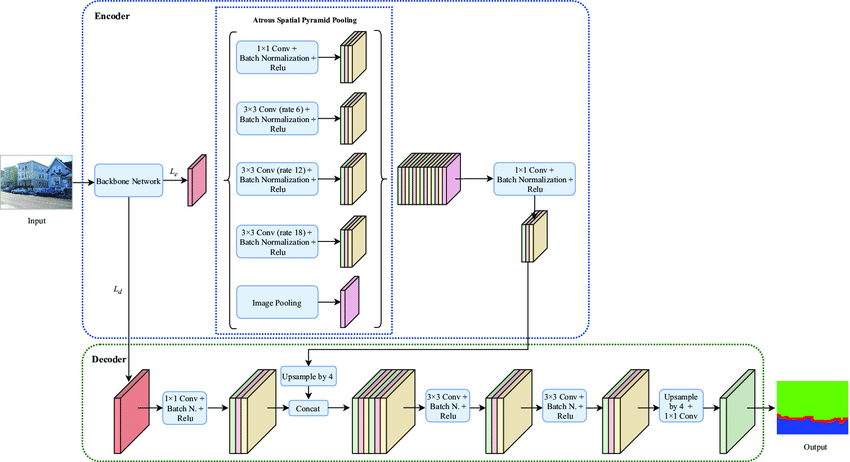
\includegraphics[width=0.6\textwidth]{Images/deeplabv3.png}
    \caption{DeepLabv3 architecture~\cite{deeplabv3-image}}
    \label{fig:deeplabv3}
\end{figure}

\begin{figure}[h]
    \centering
    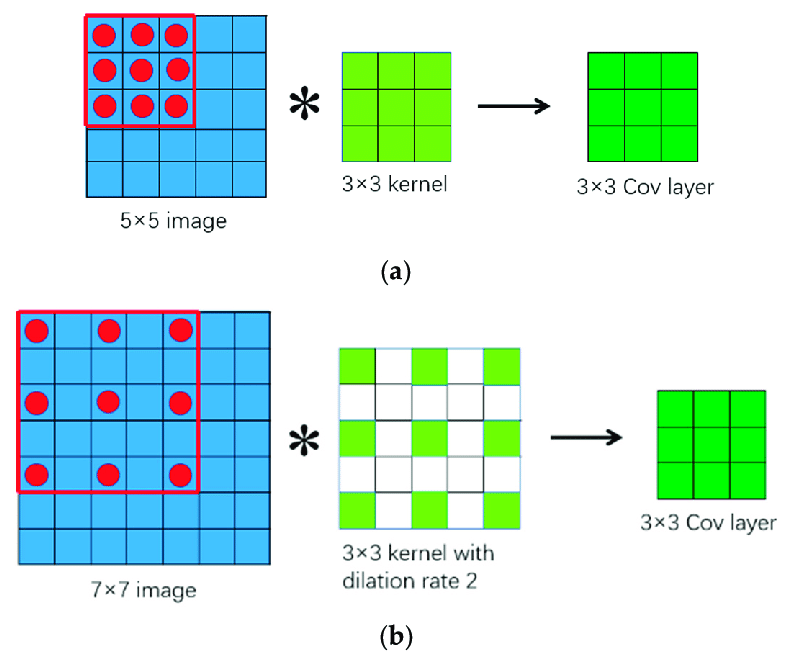
\includegraphics[width=0.5\textwidth]{Images/atrous-convolution.png}
    \caption{Atrous Spatial Pyramid Pooling (ASPP) in DeepLabv3\\ (a) Conv 3x3, rate=1 (b) Conv 3x3, rate=2 \\
    \cite{atrous-convolution-image}}
    \label{fig:atrous-convolution}
\end{figure}


\subsection{ResNet-101 Backbone}

Resnet-101 is convolutional neural network with 101 layers deep. It has residual blocks that allow the network to learn the identity function, which helps in training deeper networks. The residual blocks have skip connections that bypass one or more layers. It takes normalized RGB images as input and outputs feature maps that are used by the DeepLabv3 and the auxilary classifier. 
Input to the layer is a 4-dimensional tensor with normalized RGB channels, and the output is N*2048, where N is the batch size.  
Here, N = 1, as we are training the model with a single image at a time (small dataset).

\textbf{DeepLabv3 with a ResNet-101 backbone has approximately 53.5 million parameters.}

\begin{figure}[h]
    \centering
    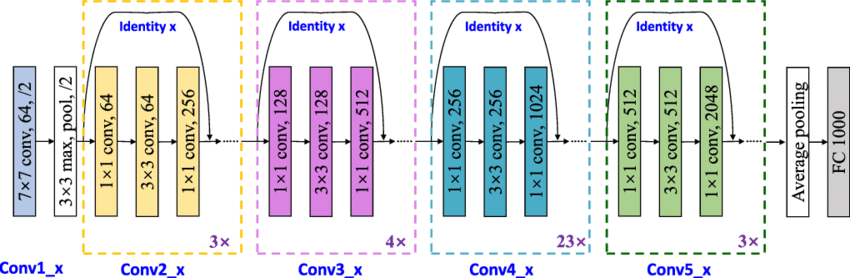
\includegraphics[width=0.5\textwidth]{Images/resnet.png}
    \caption{Residual blocks in ResNet-101 \cite{resnet-image}}
    \label{fig:resnet}
\end{figure}


\subsection{Auxilary Classifier}

The auxilary classifier is a fully connected layer that takes the feature maps from the ResNet-101 backbone and outputs a 4-dimensional tensor with the shape (N, 4, H, W), where N is the batch size, 4 is the number of classes, H is the height, and W is the width of the image. The auxilary classifier is used to improve the training of the model by providing additional supervision to the model. The output from the auxilary classifier is combined with the output from the DeepLabv3 model to improve the segmentation results.

\begin{lstlisting}
(aux_classifier):FCNHead(
(0):Conv2d(1024,256,kernel_size=(3,3),
    stride=(1, 1),padding=(1,1),bias=False)
(1):BatchNorm2d(256,eps=1e-05 momentum=0.1,
    affine=True)
(2):ReLU()
(3):Dropout(p=0.1,inplace=False)
(4):Conv2d(256,21,kernel_size=(1,1),
    stride=(1,1))
)
\end{lstlisting}{Architecture of the auxilary classifier in the model}

\subsection{Training Setup}
While training on data, the input is a 4-dimensional tensor with normalized RGB channels, and the labels are 2D tensors with integer values representing the class labels for each pixel. The output from the PyTorch model is a 4-dimensional tensor with the shape (N, 4, H, W), where N is the batch size, 4 is the number of classes, H is the height, and W is the width of the output. The output is a probability distribution over the classes for each pixel in the input image.
\\ The model is trained with the cross-entropy loss function, which is minimized using the Adam optimizer. The model is trained for 100 epochs. The learning rate is set to 0.01. The training takes approximately 30 mins to complete. The model is evaluated 3 images. The evaluation metrics used are precision, mean intersection over union (mIoU) and pixel accuracy.
